\documentclass[12pt,a4paper,fleqn]{article}
\usepackage{rmpackages}																% usual packages
\usepackage{rmtemplate}																% graphic charter
\usepackage{rmexocptce}																% for DS with cptce eval

%\cfoot{} 													% if no page number is needed
%\renewcommand\arraystretch{1.5}		% stretch table line height

\begin{document}
\normalem % makes emphasize italic again

\begin{header}
TP -- Comme un parfum de lavande (2)
\end{header}

\begin{multicols}{2}
\begin{center}
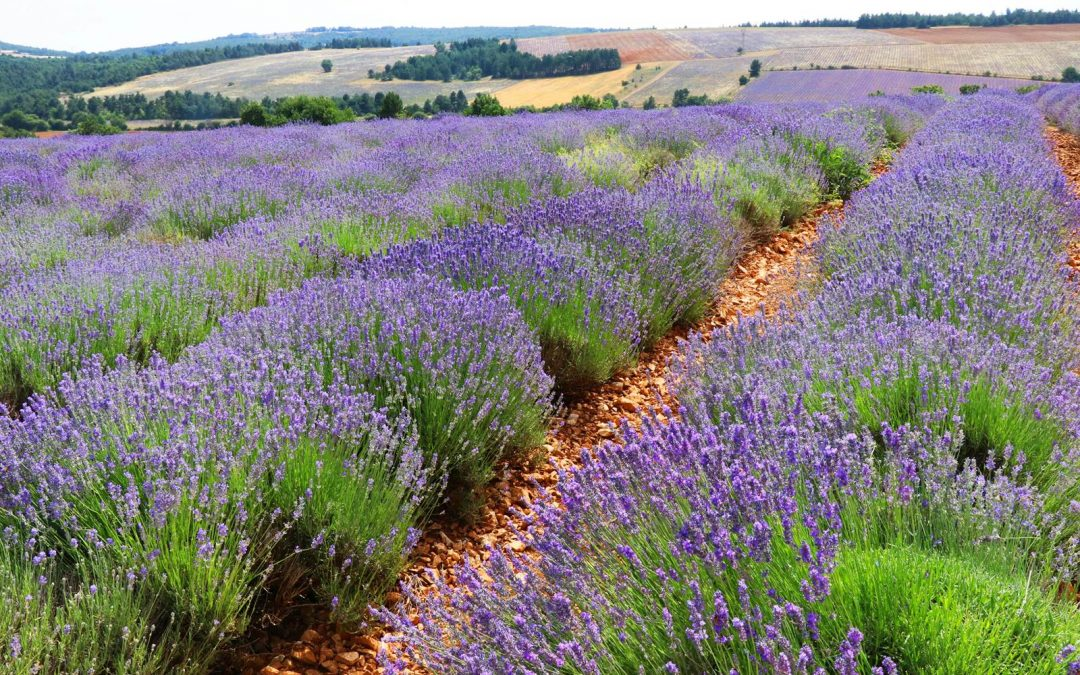
\includegraphics[width=\linewidth]{images/lavande.jpg}
\end{center}

La synthèse d'une espèce chimique doit impérativement être suivie d'une caractérisation soignée qui permet de s'assurer que le produit de synthèse correspond bien à l'espèce voulue.
C'est particulièrement vrai lorsqu'il s'agit de médicaments !

La semaine dernière, vous avez synthétisé (en principe) de l'éthanoate de linalyle.
Aujourd'hui, il faut vérifier que le produit obtenu est bien présent dans l'huile essentielle de lavande.
\end{multicols}

\begin{objectif}
Vérifier que le produit synthétisé est présent dans l'huile essentielle de lavande
\end{objectif}

\begin{doc}
\textbf{Données}
\begin{center}
\renewcommand\arraystretch{1.5}		% stretch table line height
\begin{tabular}{| >{\centering\arraybackslash}p{.15\linewidth} | *{4}{>{\centering\arraybackslash}p{.17\linewidth} |}}
\hline
 & \textbf{Linalol} & \textbf{Acétate d'éthyle} & \textbf{Éthanoate de linalyle} & \textbf{Acide éthanoïque} \\
 \hline
\textbf{Densité} & \num{0.87} & \num{0,92} & \num{0.89} & \num{1.18} \\
\hline
$T_\mathrm{ébullition}$ (\unit{\degreeCelsius}) & \num{199} & \num{77,1} & \num{220} & \num{85} \\
\hline
\textbf{Indice de réfraction} & \num{1,46} & \num{1,37} & \num{1,45} & \num{1,37} \\
\hline
\end{tabular}
\end{center}
\end{doc}

\begin{doc}
\textbf{Pictogrammes de sécurité}

Les différents produits chimiques utilisés lors de cette séance présentent certains risques qu'il faut connaitre pour s'en protéger.

\begin{center}
\begin{tabular}[c]{|l| m{5.5cm} |}
\hline
\textbf{Linalol} & 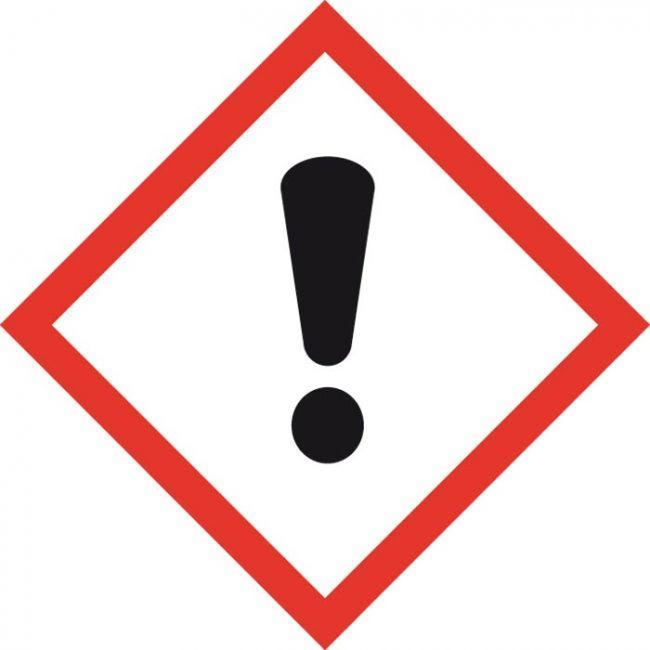
\includegraphics[trim=0 0 0 -75, height=40 pt]{images/pict_nocif.jpg} \\
\hline
\textbf{Éthanoate de linalyle} & 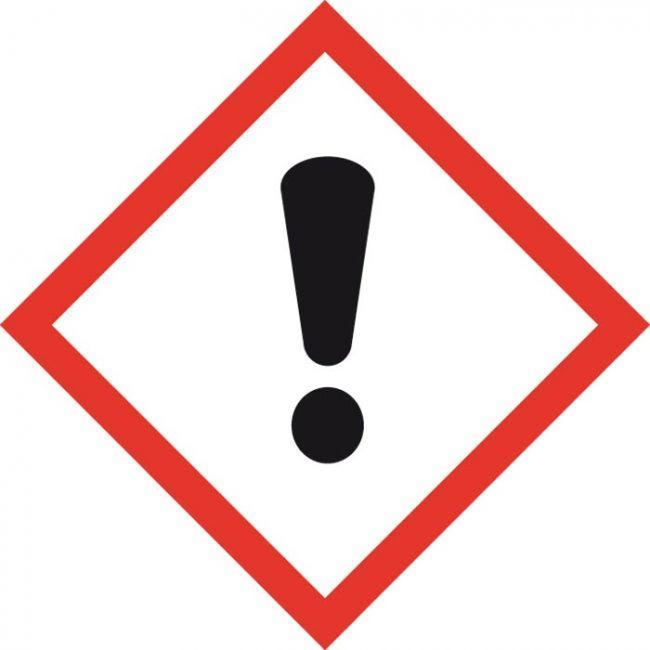
\includegraphics[trim=0 0 0 -75, height=40 pt]{images/pict_nocif.jpg} \\
\hline
\textbf{Acétate d'éthyle} & 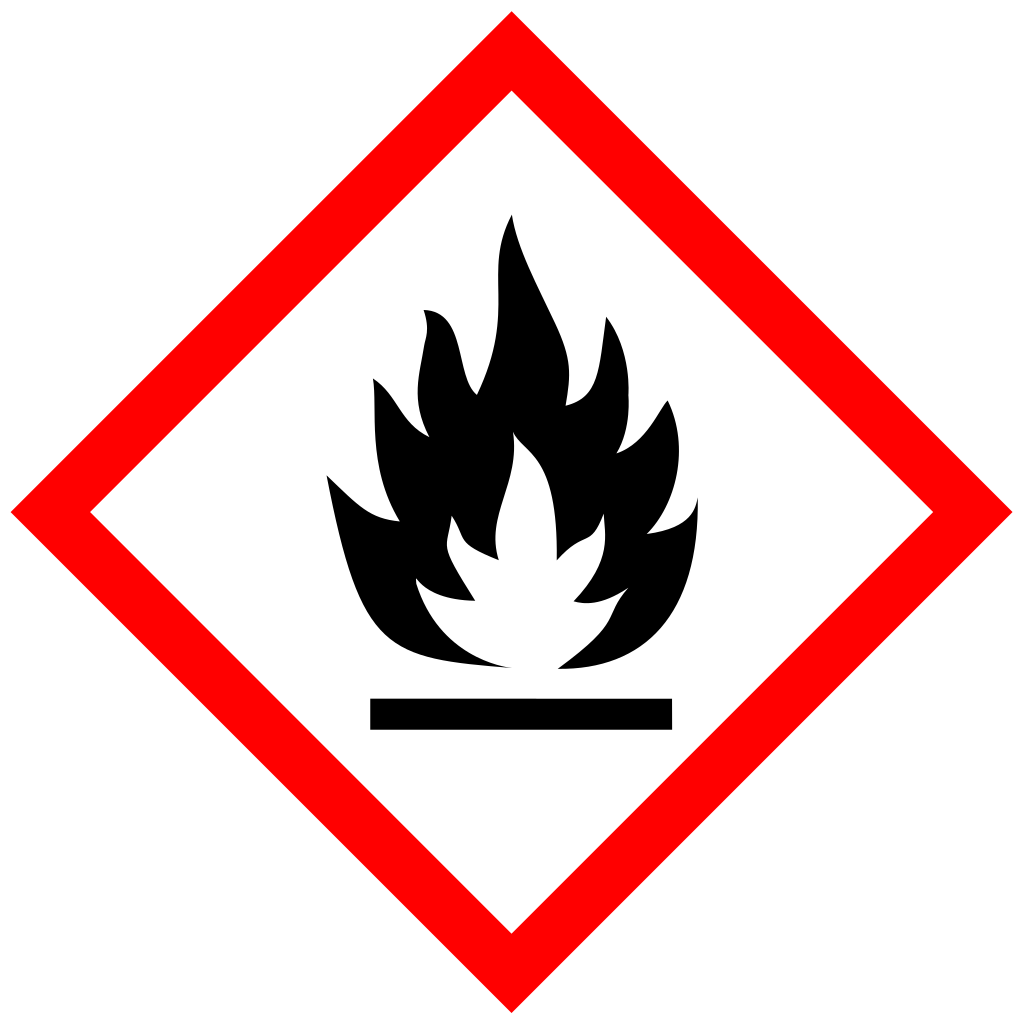
\includegraphics[trim=0 0 0 -75, height=40 pt]{images/pict_inflammable.png}  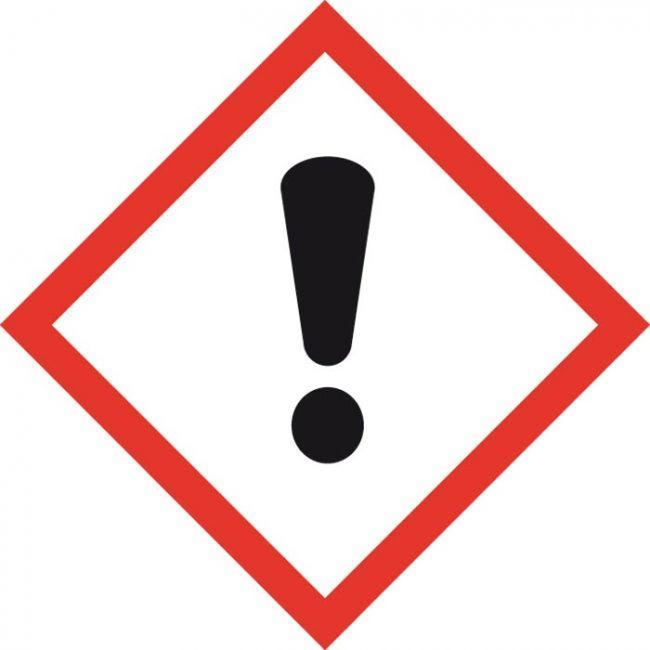
\includegraphics[trim=0 0 0 -75, height=40 pt]{images/pict_nocif.jpg} \\
\hline
\textbf{Cyclohexane} &  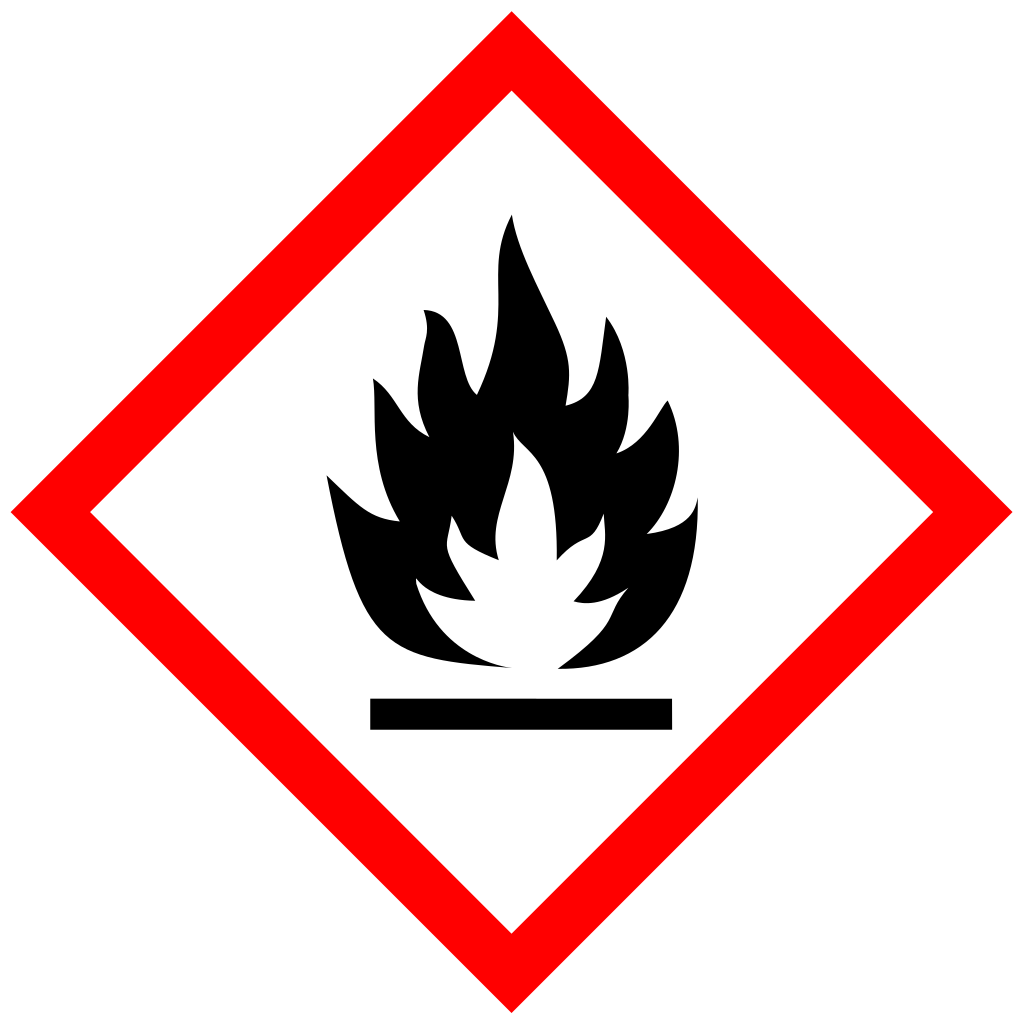
\includegraphics[trim=0 0 0 -75, height=40 pt]{images/pict_inflammable.png} 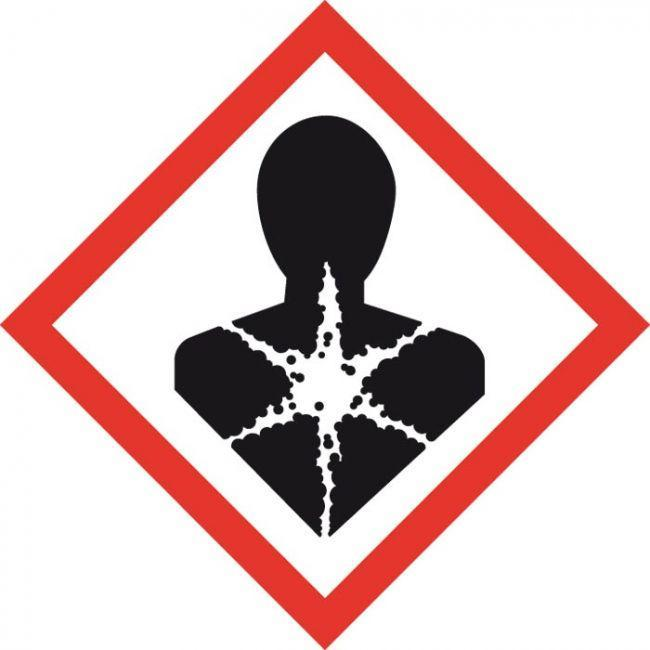
\includegraphics[trim=0 0 0 -75, height=40 pt]{images/pict_cancer.jpg}
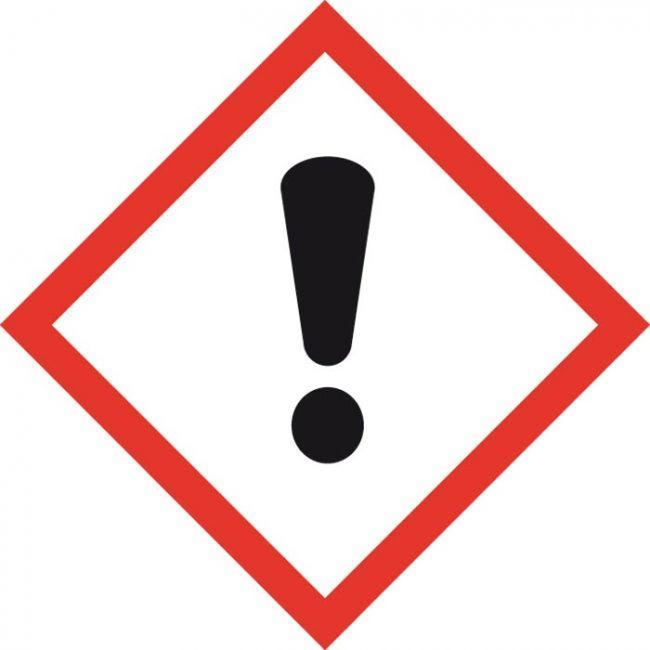
\includegraphics[trim=0 0 0 -75, height=40 pt]{images/pict_nocif.jpg} 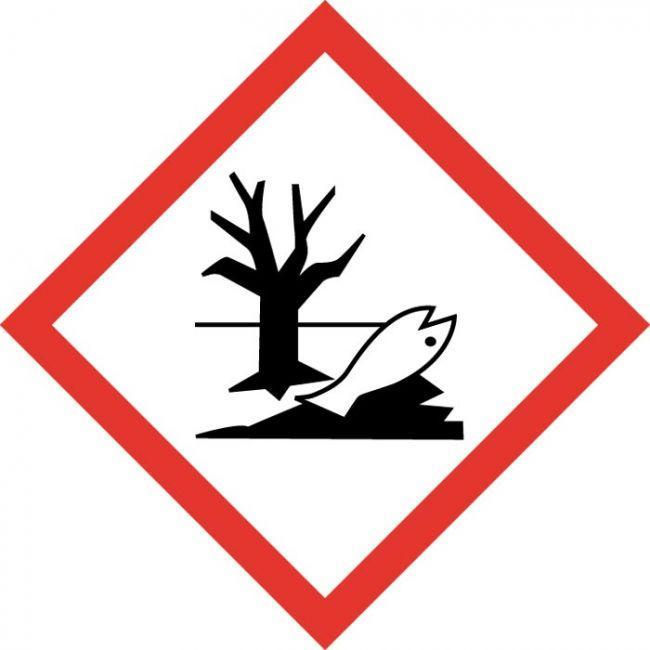
\includegraphics[trim=0 0 0 -75, height=40 pt]{images/pict_aquatique.jpg}  \\
\hline
\end{tabular}
\end{center}
\end{doc}

\begin{doc}
\textbf{Réaliser une chromatographie sur couche mince (CCM)}

Pour cette chromatographie, l'éluant est un mélange de cyclohexane (\qty{80}{\percent}) et d'acétate d'éthyle (\qty{20}{\percent}).
\textbf{\textcolor{red}{Les plaques sont fragiles ! Il ne faut pas mettre les doigts dessus et faire  preuve d'une grande légèreté lors des tracés au crayon.}}
\begin{multicols}{2}
\paragraph{Préparation de la cuve}
\begin{enumerate}
\item Verser un fond d'éluant dans la cuve : pas de plus de \qty{5}{mm} environ.
\item Fermer la cuve et patienter un dizaine de minutes : la cuve doit être saturée en vapeurs d'éluant.
\end{enumerate}
\paragraph{Préparation de la plaque}
\begin{enumerate}[resume]
\item Au crayon à papier et \textbf{sans appuyer}, tracer la ligne de dépôt à \qty{1,5}{cm} du bord.
\item Sur cette ligne, marquer trois repères régulièrement espacés.
\end{enumerate}
\paragraph{Dépôt des échantillons}
\begin{enumerate}[resume]
\item Avec un capillaire, prélever un peu de l'échantillon à déposer.
\item Déposer l'échantillon sur le repère et le noter sur une feuille.
\item Sous la lampe UV, vérifier que le dépôt est bien visible.
\end{enumerate}
\paragraph{Élution}
\begin{enumerate}[resume]
\item Sans faire de vagues, placer la plaque verticalement dans la cuve puis la refermer.
\textbf{La ligne de dépôt doit être au dessus de l'éluant !}
\item Quand le front d'éluant est à \num{1} ou \qty{2}{cm} du bord, retirer la plaque et repérer \textbf{immédiatement} le front d'éluant au crayon à papier.
\end{enumerate}
\paragraph{Révélation}
\begin{enumerate}[resume]
\item Repérer au crayon à papier la position des différentes taches visibles sous la lampe UV.
\item \emph{Optionnel : plonger la plaque une solution de permanganate de potassium puis rincer à l'eau}.
\end{enumerate}

\begin{center}
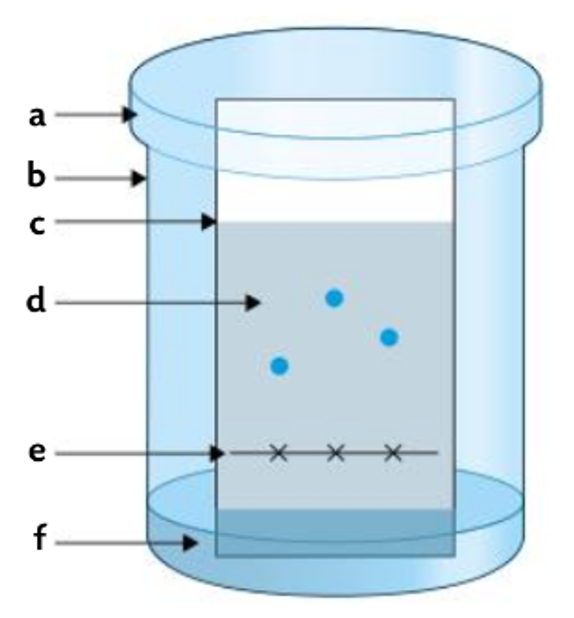
\includegraphics[width=\linewidth]{images/ccm_schema.png}
\end{center}
\end{multicols}
\end{doc}

\end{document}